%!TEX root = New.tex
\chapter{Shrink: Greening CDN Datacenters}
\label{ch:shrink}
Our growing consumption of digital content  is increasing the energy use of datacenters used for content delivery, and datacenters today consume more than 1.3\% of world's electricity consumption \cite{dcTotal}.
This growth is a result of increased availability of several forms of content such as video \cite{cisco-videogrowth,nielsen-video-growth}, and social media content, as well new platforms for content consumption, such as smartphones and tablets \cite{cisco-videogrowth}. Due to our growing dependence on digital content, mechanisms for reducing energy use of content delivery are an important societal need. 
Further, such mechanisms have potential to be an important cost-cutting tool for content delivery networks (CDNs). Energy is a major factor of operational costs \cite{barroso2007case} of a datacenter; reducing energy cost of their datacenters would help CDNs stay competitive in an commoditized marketplace.


% twin problems: 
Recent research has shown that techniques that consolidate demand in a datacenter on a subset of servers can enable turning off up to 50\% servers and bring significant energy savings \cite{mathew12,JainEnergy,lin12,lu13}. However, the impact of this energy minimization on user-perceived performance in a CDN datacenter has not been evaluated before. These studies do not evaluate how cache hit rates in a CDN datacenter would be impacted due to server shutdown policies. Note that reduced hit rates adversely affect user-perceived performance. Further, their analyses are based only in terms of system-level metrics, e.g., aggregate load at a datacenter, and not based on user-perceived metrics such as file download times. 

%it is unclear if the projected energy savings are indeed achievable without degrading user-perceived performance. 
% This is because they do not evaluate the impact of server shutdown on 
%These studies neither evaluate user-perceived metrics, e.g., file download times, or system-level metrics such as cache hit rates which are dire


The network of a datacenter, which consumes about 10-20\% of datacenter energy, can be made energy efficient by traffic engineering techniques as shown by prior work  \cite{response, elasticTree, greenTE, Chiaraviglio, Andrews}. The energy savings that a scheme achieves depends on traffic patterns in the datacenter, traffic patterns that traffic engineering schemes assume to be fixed.  This assumption isn't true for content delivery data centers, where traffic patterns could be influenced by load balancing decisions and server shutdown policies. We hypothesize that there exists potential for more network energy savings in datacenters than shown previously, provided techniques for saving server energy work in coordination with those for saving network energy. 


Our goal is to quantify how much energy savings are achievable in a CDN datacenter with minimal or no impact on user-perceived performance. 
To this end, we seek to design server and network shutdown policies that coordinate with each other and increase datacenter network energy savings,
and design server shutdown policies and load balancing algorithms that minimize the reduction in cache hit rates. To conduct a realistic evaluation of proposed techniques, we plan to collect datasets of content access traces of various types from a CDN, and  evaluate proposed strategies in terms of user-perceived metrics using a combination of trace-driven experiments and testbed experiments with a prototype.

\section{Related work}

To our knowledge, this would be first effort to evaluate energy minimizing strategies  in a CDN datacenter in terms of user-perceived performance, and to explore coordinated server and network shutdown policies.  Prior work has explored energy-minimizing strategies for datacenter and ISP networks, and has evaluated potential energy savings of datacenters, without evaluating user-perceived performance metrics.


%\textbf{Switch power management:} Nedevschi et al. \cite{Nedevschi08} study power management algorithms for switches that support sleep states or several power/performance states similar to today's CPUs. Authors show that if switches do support these features, their power management algorithms can halve the network energy consumptions for lightly loaded networks. Power management algorithms for switches, as well as in servers \cite{serverpower}, are complementary to ours, can be used along with techniques in this work.


\textbf{Energy-minimizing routing:} Several papers  \cite{response, elasticTree, greenTE, Chiaraviglio, Andrews} have proposed network energy minimizing routing algorithms for ISP networks and data center networks.   These approaches save energy by  concentrating the traffic, which is input in the form of a traffic matrix, on a subset of links and switches, and shutting off remaining switches and links. In \cite{response} and \cite{elasticTree}, authors demonstrate using Click and OpenFlow based prototypes respectively, the feasibility of implementing these routing protocols in today's switches. In comparison to approaches that optimize routing for a given traffic matrix, this work explores how server shutdown policies can coordinate with energy-minimizing routing strategies to increase energy savings in a datacenter.
% coordinated optimization of content placement and routing for a CDN datacenter that can yield greater network energy savings.

%These approaches assume that both endpoints of a flow are fixed, while in the context of content-serving clusters,  any available server can act as the source of a flow. 
% The flexibility of choosing the source allows greater network energy savings compared to approaches that optimize routing for a given traffic matrix.
%********* add work on data-center traffic engineering *********

\textbf{Energy-proportional datacenters:} Analysis of data center traces have shown that servers in datacenters are  lightly loaded in many cases. Motivated by this observation, several papers \cite{mathew12,JainEnergy,lin12,lu13}, based on trace-driven experiments, have explored how much energy savings can be obtained by using only a fraction of the servers at a given time, and by shutting-off remaining servers or switching them to a low power state. 
%Their goal is to estimate  the fraction of servers to be kept in active state to handle the demand at any given time, while also limiting the frequency of transitions between different power states to reduce server wear-and-tear. 
While these studies show that there is significant potential for energy savings, they implicitly assume the total load will be evenly distributed among the active set of servers. However, server shutdown policies could cause additional load imbalance in datacenters, thereby degrading user-perceived performance. Further, in case of a CDN datacenter, they do not evaluate the impact of server shutdown policies on cache hit rates, which are a key determinant of user-perceived performance. In comparison, a key goal of this work is to design load-balancing and server shutdown strategies that ensure cache hit rates are minimally affected, and load imbalance is small enough to not cause a degradation in user-perceived performance.

\textbf{Other work:} There are a number of recent efforts whose goals are complementary to this work. Work on device-level power management for switches \cite{Nedevschi08} and servers \cite{serverpower} could complement our strategies. A CDN could use geographic load balancing to globally optimize energy use across  datacenters while using our strategies in a single datacenter \cite{qureshi2009cutting,Liu11,Gao12,Rao10}. Using recently developed techniques for designing highly scalable load-balancers such as ETTM \cite{ettm} and  Ananta \cite{ananta}, a CDN can extend the strategies we propose in this work to develop a scalable solution for use in datacenters with tens of thousands of servers.

%These papers implicitly assume that the total load across servers is independent of the fraction of servers that are active,  and that the load will be evenly distributed across the active set of servers. A key goal of this work is to show how these properties can be satisfied for CDN datacenters.

%First,  we orchestrate movement of content before server shutdown and after server startup events to ensure that cache hit rates are minimally affected before and after server shutdown and startup events. Second, we make content placement and redirection decisions to evenly distribute the load across the active servers.  

%**** Also, add no network. *****

%****** dig up data on P state and C state ******

%****** experiment with DVFS ******


%These papers propose algorithms  to save server energy use in a cluster by shutting-off or switching to a low power state a fraction of servers, while (i) keeping 

%For content-serving clusters, the load on a server depends on cache how often a server is able to serve content from its local cache and cannot be assumed to be constant, and for load to be evenly distributed across servers, content placement algorithms must be suitably designed as we show in this paper.


%\textbf{Energy-reduction via geographic load-balancing:} Many papers \cite{qureshi2009cutting,Liu11,Gao12,Rao10} have shown that geographical load-balancing across data centers can exploit the differences in electricity prices and in renewable energy availability at various locations to reduce energy costs,  energy use, or non-renewable energy use. In comparison, our work focus on improving energy-efficiency of a single cluster by maximizing shut-down periods of servers and network components by  suitably designing placement and routing algorithms.


%\textbf{Load-balancing algorithms:}  Consistent-hashing based replication techniques \cite{consistent-hashing,chord,dynamo} have been used widely to build applications where load-balancing and fault tolerance are required. If a high percentage of servers have been made inactive to save energy then naively applying these techniques could result in highly unbalanced load across servers. In this work, we will study how consistent-hashing based techniques can be adapted to provide load-balancing when a large number of nodes are inactive.  

%\textbf{Load-balancing systems:} State-of-the-art load balancing systems such as ETTM \cite{ettm} and  Ananta \cite{ananta} provide a scalable load-balancing solution by moving stateful packet-processing functionality, e.g., NAT translation, to the end-hosts. Our work focuses less on the scalability of the load-balancing system, and more on designing load-balancing policies that reduce cluster energy use by allowing a large fraction of servers and network components to be shut off.

%\textbf{Leveraging placement flexibility:} Choudhary et al. \cite{Chowdhury}  show that cluster file systems, e.g., HDFS, GFS, etc., can leverage the flexibility to choose the destination of their writes to avoid congested network links and improve write latencies. Sharma et al \cite{beyondmlu} show that location diversity of content in ISP networks can significantly enhance the performance of traffic engineering algorithms. In the context of  network CDNs, Sharma et al \cite{NCDN} show that content placement flexibility is a powerful degree of freedom and effective content placement in combination with simple static routing algorithms gives close to optimal results for traffic engineering and content distribution objectives. 
%*** none of them consider energy minimization *** 



\section{Research outline}

Our goal is to design a comprehensive solution for CDN datacenters which makes load balancing, server shutdown, and traffic engineering decisions to reduce energy use with a minimal impact on user perceived performance. 


\begin{figure}
\centering
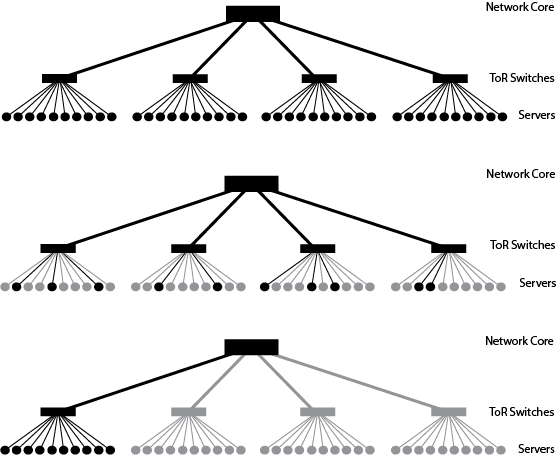
\includegraphics[scale=0.4]{energy/dcTopology.png}
\label{fig:server-network}
\caption{A datacenter topology. Black components are turned on and grey components are turned off. (Top) All servers and switches are on as is the current practice. (Middle) Demand is consolidated on randomly selected 10 servers and remaining servers are shutoff. All ToR switches must be kept on to provide connectivity to servers. (Bottom) Demand is consolidated on servers in one rack, which allows  servers as well as ToR switches in other racks to be turned off.}
\end{figure}


\begin{figure}
\centering
\vspace{-0.3in}
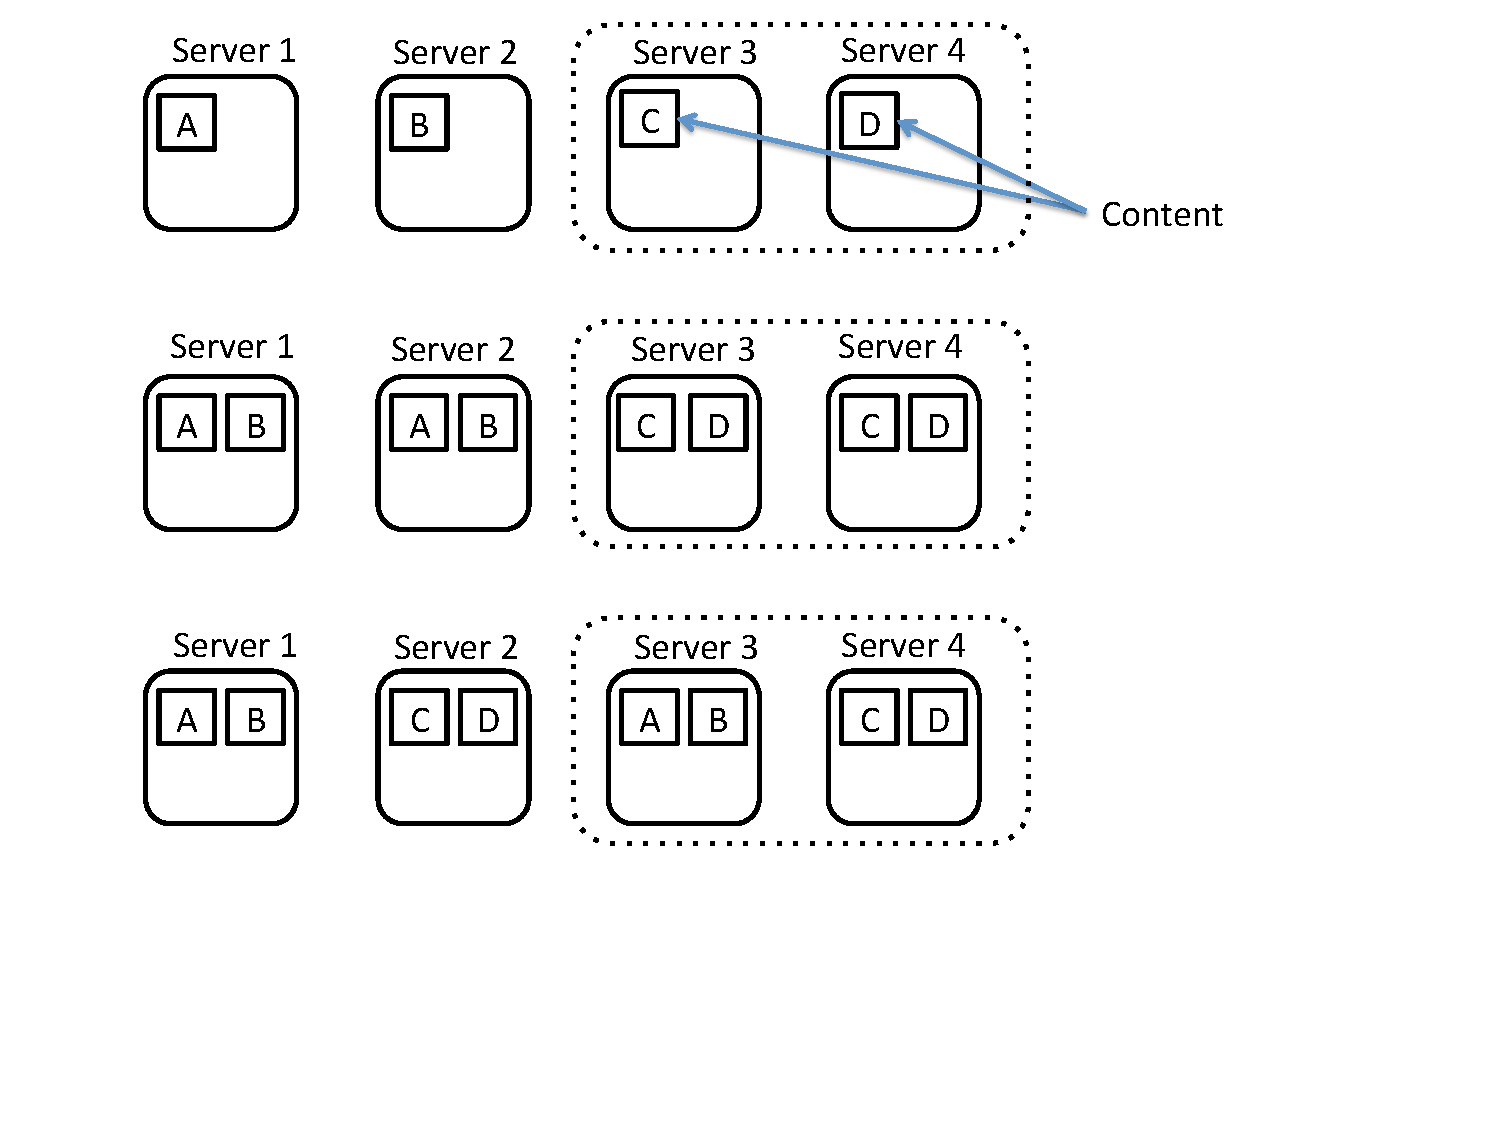
\includegraphics[scale=0.5]{energy/server-content.pdf}
\label{fig:server-content}
\vspace{-0.8in}
\caption{Replication strategy impacts content availability after server shutdown. All four servers are active during normal utilization periods, but the two servers on the right are turned off during low utilization periods. Squares with same letters represent replicas of the same content. (Top) One replica of each content is maintained as shown. When servers 3 and 4 are shutdown, two of the four content become unavailable. (Middle) Two replicas of each content are maintained,  but still shutting down servers 3 and 4 makes two of the four content unavailable. (Bottom) Two replicas of each content are maintained, but servers 1 and 2 have one copy of all four content. In this case, all content is available despite shutting down servers 3 and 4.}
\end{figure}


\subsection{Algorithm design}
\label{sec:shrinkalgo}
There are three design questions which are key to achieving the performance and energy-efficiency goals of a CDN datacenter.

\textbf{(1) How many servers to keep active?} 
Reducing the number of active serves is necessary for energy-efficiency because servers consume more than 80\% of power usage in datacenters \cite{Abts2010}, and today's servers consume 50-70\% energy even in idle state \cite{barroso2007case}. 
We will decide the number of active servers to ensure the following:

\noindent\emph{Availability:} The datacenter will have sufficient  resources, e.g, compute, network, disk bandwidth, to handle all incoming requests.
ensure both high availability  and high performance. 

\noindent\emph{Performance:} Cache misses at datacenter require objects to be fetched from a remote datacenter and results in a noticeable increase in user-perceived performance. The aggregate storage available across servers will be sufficient to enough a cache hit rate that is comparable to the cache hit rates if all servers were active. 

%To ensure availability, the number of servers is chosen so that there are sufficient  resources, e.g, compute, network, disk bandwidth, to handle all incoming requests.
%
%For high performance 
%%We will keep sufficient number of servers active so that there are sufficient  resources, both compute and network, to handle all incoming requests.
%To ensure availability, we will keep sufficient number of servers active so that 
%(1) there are enough compute resources available across servers to handle incoming request rate and (2) 
%The second criteria is necessary because cache misses at datacenter require objects to be fetched from a remote datacenter and results in a noticeable increase in user-perceived performance. 

\textbf{(2) Which servers to keep active?}
The set of active servers determine the potential  energy savings�from network switches. As shown in Figure \ref{fig:server-network}, randomly selecting the set of active servers requires entire datacenter network to be turned off. Therefore, we will select the active servers in a manner that enables more network switches to be turned off, e.g., selecting servers that are within a small sub-tree in a datacenter topology. 

\textbf{(3) Which servers to replicate each content?}
As Figure \ref{fig:server-content} shows, if insufficient number of replicas are maintained or the set of servers is not chosen carefully, then server shutdown could  temporarily make content unavailable in the cluster. Such content unavailability decreases cache hits in datacenter, thereby hurting user perceived performance. 
To maximize cache hits, we will replicate content across servers so that  despite ongoing server shutdown events,  one copy of content is kept available in most cases.



\subsection{System overview}
\label{sec:shrinksystem}
Our algorithms would be implemented as a datacenter manager software, called \textbf{\shrink}, running at the front-end load balancer. All servers in the datacenter would be running a caching proxy software such as Squid \cite{squid}. All caching proxies would be configured as peers of one another, enabling them to request content from one another. 
\shrink\ would make its decisions based on content demand statistics from each server. To this end, \shrink\ would require support from daemon processes running at each server for reporting statistics. 
Periodically, \shrink\  would  compute load balancing and  traffic engineering decisions, and also decide which set of servers and switches to keep active in the next interval. The computed load balancing decisions would be updated locally.  To implement routing decisions, \shrink\ would require OpenFlow \cite{openFlow} support at switches to communicate the computed routing. To turn servers on/off as necessary, \shrink\ would again depend on the daemon process running at each server.
%\shrink\ would informs switches of the updated routing decisions, and would inform servers. 
%The functionality to support powering on/off switches and servers is implemented via TBD and TBD respectively. 
%Based on content demand statistics from servers, 




\subsection{Data collection}
To evaluate  our strategies for a realistic content workload, we have collected content access traces from a datacenter of a leading commercial CDN, Akamai. The traces include all requests received at a datacenter with 18 servers over a week in December 2013. Our anonymized traces traces include several major types of traffic observed in a CDN including video, social media, and other web traffic. Each anonymized log entry includes among other fields, the request timestamp, content URL, size of requested content, actual number of bytes sent, and IP address of the user. Overall, the traces contain more than 2 billion requests generating nearly 200 TB of network traffic.


\subsection{Experimental evaluation}
Our experimental evaluation would seek to find answers to following questions:
\begin{itemize}
\item
How much energy savings do our strategies achieve compared to the current practice of leaving entire datacenters in ``always on'' state? How does it compare with respect to a lower bound on energy savings?
\item
How do the user-perceived performance metrics such as file download times impacted compared to an ``always on'' strategy?  What, if any, is the increase in average and 99-percentile latency? Does a specific subset of content, such as that of a single content provider, see a performance degradation?
\item
How much additional energy saving does a coordinated server and network shutdown save over uncoordinated approaches for different datacenter network topologies?
\end{itemize}

A timeline of the proposed research for this project is given in Chapter \ref{ch:proposed}.

%
%
%\subsection{Timeline}
%The proposed research would be conducted in two phases as outlined below.
%
%\textbf{Algorithm design and trace-driven evaluation (2 months):} Our first goal would be to design algorithms for problem in Section \ref{sec:shrinkalgo} and iteratively refine them by conducting trace-driven evaluation with our datasets. Trace-driven evaluation can be accomplished faster than actual experimentations, and will help us iterate quickly over our algorithms.
%
%\textbf{Prototype development and evaluation (2 months):} The second phase would involve a developing research prototype, whose main components are following: \textbf{(1) Shrink core:} This module would implement the algorithms designed in the first phase, namely those for deciding the set of active elements in a datacenter, and determining network routing and load balacing decisions.  \textbf{(2) Server and switch daemons:} The role of server and switch daemons is discussed in Section \ref{sec:shrinksystem}. These daemons could be integrated within a process already running at that server, e.g., the proxy software \cite{squid}, or may be implemented as a stand-alone processes.  \textbf{(3) Client:} The client module will send HTTP requests to simulate a datacenter workload and measure end-to-end performance.
%
%%\textbf{(4) Control module:} Its function would be to start and stop each of the above components during an experiment evaluation. 
% 
%We plan to conduct an experimental evaluation with the above prototype on a cloud platform, e.g, Amazon EC2 \cite{amazonec2}, as well on the 12-node Skuld cluster within our department. We expect the experiment evaluation to be an iterative process as well in which experimental findings lead us to reconsider both the designed algorithms and the system implementation.
%
%
